\documentclass[landscape]{article}
\usepackage[a4paper,landscape,margin=1.5cm]{geometry}
\usepackage{graphicx}
\usepackage{array}
\usepackage{tabularx}
\usepackage{colortbl}
\usepackage{xcolor}
\usepackage{fancyhdr}
\usepackage{tikz}
\usepackage{booktabs}
\usepackage{subcaption}
\usepackage{pagecolor}

\graphicspath{{illustration/}{reference/}}  % DO NOT CHANGE THIS LINE

% Define custom colors
\definecolor{headerred}{RGB}{255,0,0}
\definecolor{lightgray}{RGB}{240,240,240}
\definecolor{lightbeige}{RGB}{252,250,245} % Light beige color
\pagecolor{lightbeige} % Set background color

% Custom page style
\pagestyle{fancy}
\fancyhf{}
\renewcommand{\headrulewidth}{0pt}
\cfoot{\textcolor{headerred}{\thepage}} % Added page number in footer center

\begin{document}
% Header Section
\begin{center}
\Huge\bfseries\sffamily\textcolor{headerred}{TECHNICAL SPECIFICATION SHEET}
\end{center}

\vspace{0.5cm}

% PRODUCT DETAILS
\noindent\begin{tabularx}{\textwidth}{|X|X|X|X|}
\hline
\rowcolor{headerred}\multicolumn{4}{|c|}{\textcolor{white}{\textbf{PRODUCT DETAILS}}} \\
\hline
Brand Name: W & Designer: J & Season: Spring/Summer & Category: Casual \\
\hline
Date: \today & Style Name: Modern Code & Style Number: C123 & Main Fabric: Cotton \\
\hline
\end{tabularx}

\vspace{0.5cm}

% STYLE DESCRIPTION
\noindent\begin{tabularx}{\textwidth}{|X|}
\hline
\rowcolor{headerred}\multicolumn{1}{|c|}{\textcolor{white}{\textbf{STYLE DESCRIPTION}}} \\
\hline
This piece features a modern, casual design with a focus on comfort and versatility, crafted from lightweight cotton.
\end{tabularx}
\hline

\vspace{0.5cm}

% TECHNICAL DRAWINGS
\noindent\begin{tabularx}{\textwidth}{|X|}
\hline
\rowcolor{headerred}\multicolumn{1}{|c|}{\textcolor{white}{\textbf{TECHNICAL DRAWINGS}}} \\
\hline
\begin{center}
% First row of drawings
\begin{tabular}{ccc}
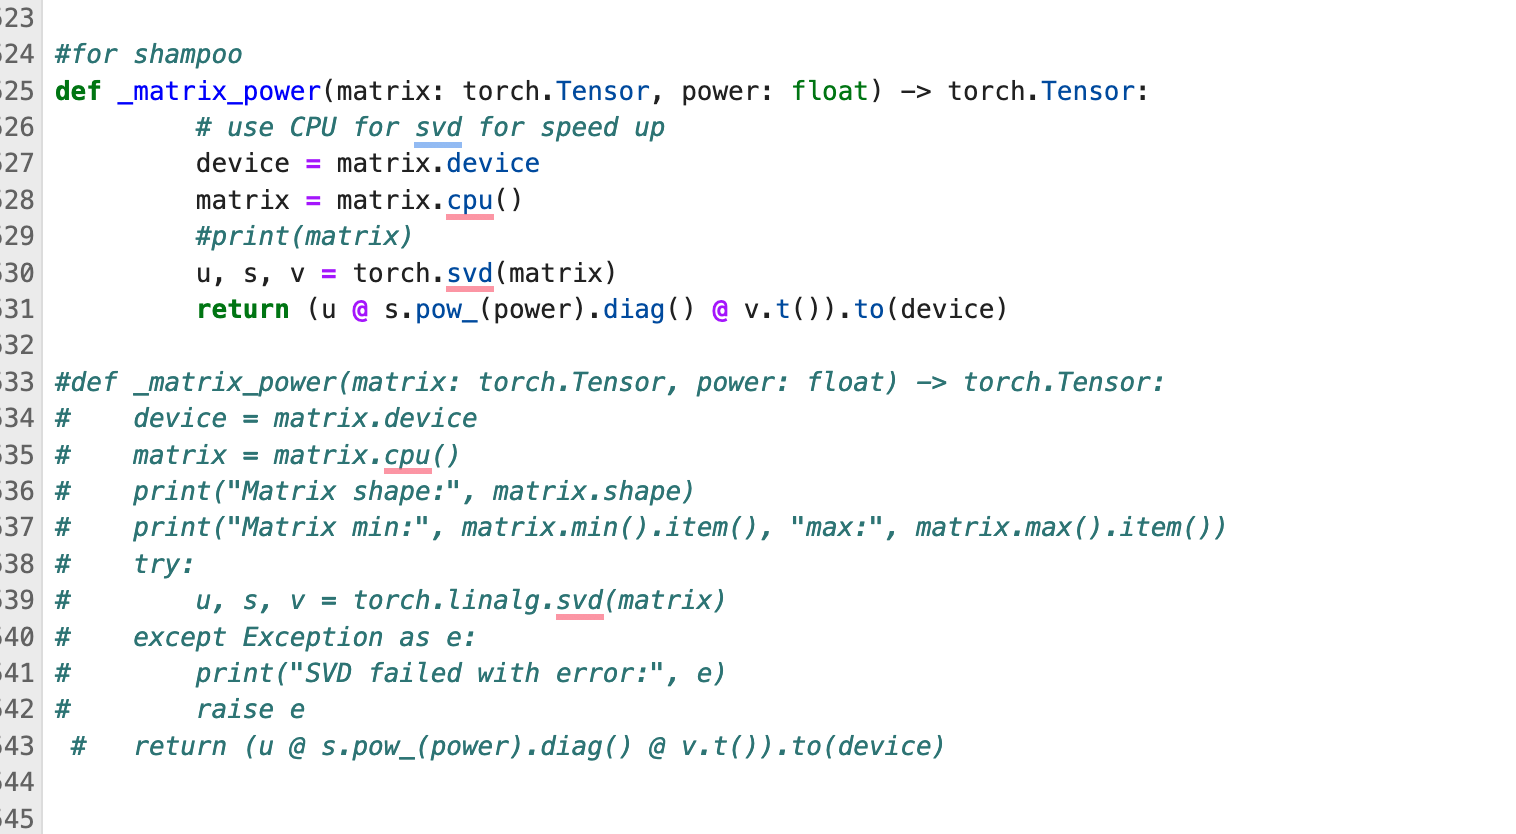
\includegraphics[width=0.4\textwidth,height=8cm,keepaspectratio]{Screenshot_2025-03-09_at_15.26.02.png} &
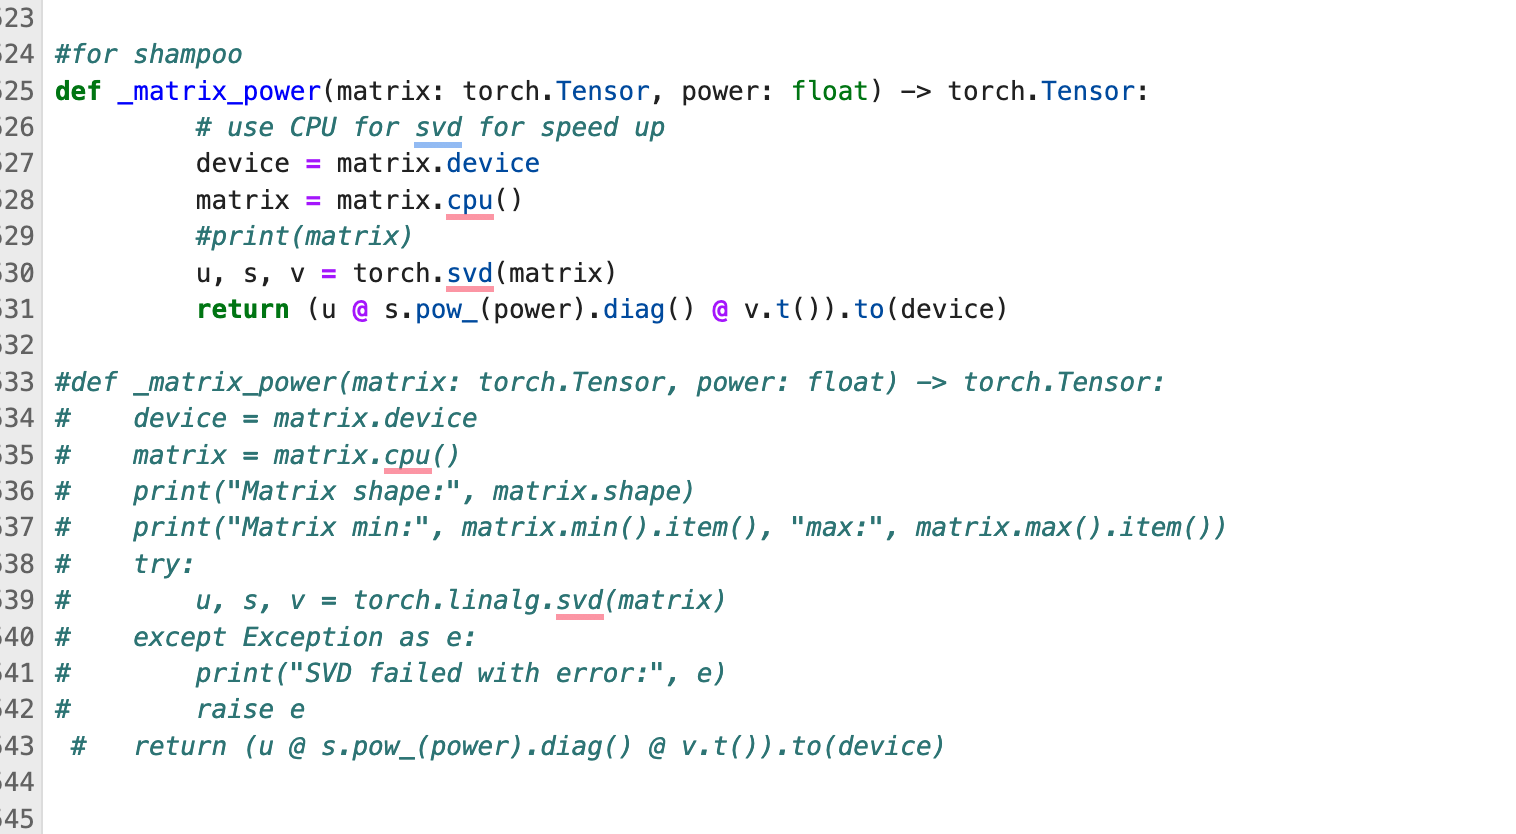
\includegraphics[width=0.4\textwidth,height=8cm,keepaspectratio]{Screenshot_2025-03-09_at_15.26.02.png} &
\end{tabular}
\end{center}
\end{tabularx}
\hline

\vspace{0.5cm}

\newpage
% MEASUREMENTS
\noindent\begin{tabularx}{\textwidth}{|X|X|X|X|X|X|X|}
\hline
\rowcolor{headerred}\multicolumn{7}{|c|}{\textcolor{white}{\textbf{MEASUREMENTS}}} \\
\hline
\textbf{Item} & \textbf{Description} & \textbf{XS} & \textbf{S} & \textbf{M} & \textbf{L} & \textbf{XL}\\
\hline
Shoulder & Width from seam to seam & 38 cm & 40 cm & 42 cm & 44 cm & 46 cm \\
\hline
Chest & Circumference around chest & 90 cm & 95 cm & 100 cm & 105 cm & 110 cm \\
\hline
Length & From shoulder to hem & 60 cm & 62 cm & 64 cm & 66 cm & 68 cm \\
\hline
\end{tabularx}

\vspace{0.5cm}

% CARE INSTRUCTIONS
\noindent\begin{tabularx}{\textwidth}{|X|}
\hline
\rowcolor{headerred}\multicolumn{1}{|c|}{\textcolor{white}{\textbf{CARE INSTRUCTIONS}}} \\
\hline
\begin{itemize}
\item Machine wash cold, gentle cycle.
\item Do not bleach.
\item Tumble dry low.
\item Iron on low heat if necessary.
\item Dry clean optional.
\end{itemize}
\end{tabularx}
\hline

\vspace{0.5cm}

% ADDITIONAL COMMENTS
\noindent\begin{tabularx}{\textwidth}{|X|}
\hline
\rowcolor{headerred}\multicolumn{1}{|c|}{\textcolor{white}{\textbf{ADDITIONAL COMMENTS}}} \\
\hline
% INSERT ADDITIONAL COMMENTS HERE
\end{tabularx}
\hline

\end{document}